\section{Simulation Results}
\label{sec:results}

\subsection{Baseline Results}

The model with the described implementation has been tested on the Sioux-16 network
with a flow capacity scaling 0f $70\%$ to allow for a reasonable amount of congestion.

The travel disutility parameter has been chosen to be zero, as is the travel
disutility for taking a car in Sioux-16. The reason behind this is that there are
numerous studies indicating positive and negative effects of autonomous vehicles, so
it is hard to decide whether the perception of AVs will tend towards one side or the
other compared with cars. To name just two examples, it has been stated that autonomous
vehicles will increase the usefulness of time spent in the car, because people will
be able to do work \todo{cite sth}. On the other hand it has been found that people
are most likely to suffer from travel illness if they aren't concentrating on the
road \todo{cite sth} and people subjectively might perceive the travlel in an AV
as lasting longer compared to the car, due to the lack of activity.

The constant disutility for cars in the Sioux scenarios
has been computed by combining the travel disutility for 10min walking (as to
account for getting to and from a parking lot) and the monetary disutility for
paying \$6 for parking. For the AVs in this simulation it has been assumed that
there is no such additional cost, but a monetary fee per taking an AV trip. This
assumes that a fictious operator already included the costs of parking into the
pricing theme (which is reasonable taking the values form actual taxi services).

Since the values in Sioux-14 are based on measurements in Sydney, the current
maximum charges for taxi trips there have been used as a reference \citep{NSW2016}. According to this
source an initial charge of \$3.60 has been added to the constant disutility, while
the monetary distance factor for AVs has been set to \$2.19 per km.

Finally, the disutility for waiting for an AV has been assumed to be the same as
the waiting disutility for publci transport from Sioux, which itself is just a
vague assumption, but at least allows for a systematic comarison.

\begin{table}[]
\centering
\caption{Baseline Scenario Parameters}
\label{tab:baselineparams}
\begin{tabular}{@{}lll@{}}
\toprule
Parameter                       & Computation & Baseline Value \\ \midrule
Constant Utility per Trip       & $C_{av} = -\beta_m \cdot \$3.60$    & $-0.2232$ \\
Marginal Utility of Travel Time & $\beta_{trav,av} = \beta_{trav,car}$            & $0.0$ \\
Monetary Distance Rate          & $\gamma_{car} = 2.19 \$/km $            &  $0.00219$              \\
\midrule
Marginal Utility of Wait Time   & $\beta_{wait,av} = \beta_{wait,pt}$            &  $-0.18$              \\ \bottomrule
\end{tabular}
\end{table}

Using these parameters, which are summarized in \cref{tab:baselineparams}, the
scenario has been simulated until relaxation. The following paragraphs will show
the respective results in terms of the traffic situation. A sufficiently high
number of available AVs ($N=8000$) to show how agents make a choice for taking
an AV based on their utility evaluation.

Table \cref{tab:withwithoutav} shows the basic trip statistics of the case where
AVs have been introduced to the baseline scenario. It can be seen that with the
given utility parameters, the AVs reach a share of almost $30\%$ averaged over
the day, mainly decreasing the share of public transport and walking, while also
attracting some of the former private car users.

Interesting to see is that for public transport and walking agents the travel
distances decrease, because relatively long trips in those modes will be replaced
by AVs, thus drawing the average down to shorter trips, while it increases for cars.
Here, mainly the shorter car trips are replaced by AVs.

These results can also be in \cref{fig:modehist_av}, where the distribution of
travel distances by mode is presented. Clearly, AVs act as a competitor towards
public transport there, serving mainly the same range of trips with the assumed
utility parameters.

\begin{figure}
    \centering
    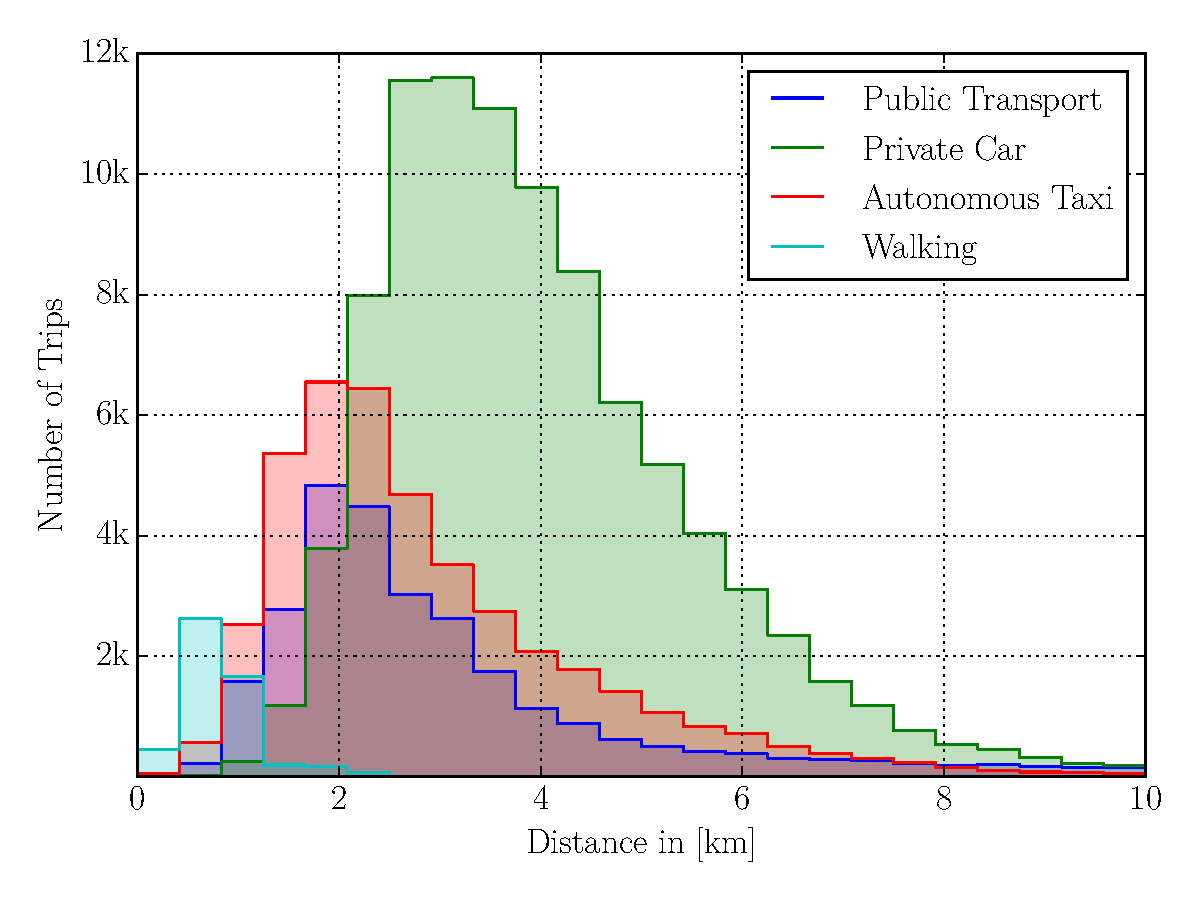
\includegraphics[width=1.0\textwidth]{figures/modehist_av.pdf}
    \caption{\todo{todo}}
    \label{fig:modehist_av}
\end{figure}

In terms of travel times it can be seen that there is a slight increase for the car
mode, which stems from the same argument as before. The decrease in travel time for
public transport and walking agents is quite significant though. For the walking
agents the change is obvious as described before. The decrease for public transport
can be explained by the switch of agents, who needed to have long walking distances
to the closest bus stop, which is included in the calculation. By only keeping those
agents at using public transport, which live nearby a bus stop, the overall travel
time decreases quite substantially.

% Please add the following required packages to your document preamble:
% \usepackage{booktabs}
\begin{table}[]
\centering
\caption{\todo{TODO, formatting}}
\label{tab:withwithoutav}
\begin{tabular}{@{}lll@{}}
\toprule
                                   & \textbf{Baseline} & \textbf{With AV} \\ \midrule
\textbf{Travel Distances {[}km{]}} &                   &                  \\
Car                                & 3.74              & 4.13             \\
Walking                            & 1.27              & 0.80             \\
Public Transport                   & 3.86              & 3.27             \\
Autonomous Taxi                    &                   & 2.78             \\
\textbf{Travel Times {[}mm:ss{]}}  &                   &                  \\
Car                                & 06:59             & 08:26            \\
Walking                            & 25:19             & 16:02            \\
Public Transport                   & 28:32             & 19:56            \\
Autonomous Taxi                    &                   & 10:08            \\
\textbf{Mode Shares}               &                   &                  \\
Car                                & 64.84\%           & 52.54\%          \\
Walking                            & 6.80\%            & 2.81\%           \\
Public Transport                   & 28.36\%           & 15.79\%          \\
Autonomous Taxi                    &                   & 28.85\%          \\ \bottomrule
\end{tabular}
\end{table}


Table \cref{tab:basemodeshares} shows how the mode choice took place after AVs
have been introduced. The rows show the original modes, while the percentages
indicate how many of the initial users were using the column mode after the
introduction of AVs. What can be seen is that $46\%$ of all initial public transport
users and $60\%$ of all walking people opted for taking an AV, while only $18\%$
of car users switch modes. This again shows that with the baseline parameters, AVs rather
work as a competitor against public transport while additionally drawing new adopters
from the walking people. Therefore this scenario represents the rather unwanted case
where AVs actually lead to a less optimal situation on the road, leading to more
congestion and less use of collective transportation.

% Please add the following required packages to your document preamble:
% \usepackage{booktabs}
\begin{table}[]
\centering
\caption{\todo{TODO}}
\label{tab:basemodeshares}
\begin{tabular}{@{}lllll@{}}
\toprule
                 & Autonomous & Car     & Public Transport & Walking \\ \midrule
Car              & 17.72\%    & 80.65\% & 1.53\%           & 0.10\%  \\
Public Transport & 46.71\%    & 0.80\%  & 51.93\%          & 0.56\%  \\
Walking          & 60.54\%    & 0.30\%  & 1.14\%           & 38.02\% \\ \bottomrule
\end{tabular}
\end{table}

The waiting times for AVs are on average around 04:40 min in the morning peak
and 02:55 min in the afternoon, while the daily average lies at 01:40 min.

In terms of travel distances the total amount of kilometers driven increased from around 404,000 km in
the baseline to 527,000 km in the AV scenario. The amount of kilometers driven by AVs
is 161,000 km from which around 29,000 are for the purpose of picking up passengers, i.e.
they are unoccupied during this time, which is roughly $18\%$. This is quite a small number
compared to ordinary taxi services. This is quite small compared to ordinary taxis with
52\% as stated in recent statistics for Oslo \citep{Norway2015} or around 50\% in Barcelona
\citep{Amat2014}.

Finally, \cref{fig:avwork} shows the states of the AVs during the day. While the
lines show how many AVs are currently performing either a pickup or dropoff task,
i.e. being ``en tour'', the shaded areas show how many passengers have been picked
up or dropped off at at certain time of the day. In this baseline scenario, only
around 3000 cars are actually active of the available 8000, so from the perspective
from an AV operator the scenario also would not be an ideal case, because the
usage of the AVs is not nearly close to saturation.

This following section will show how perturbations to the given parameters will
change the system behaviour of the simulation.

\begin{figure}
    \centering
    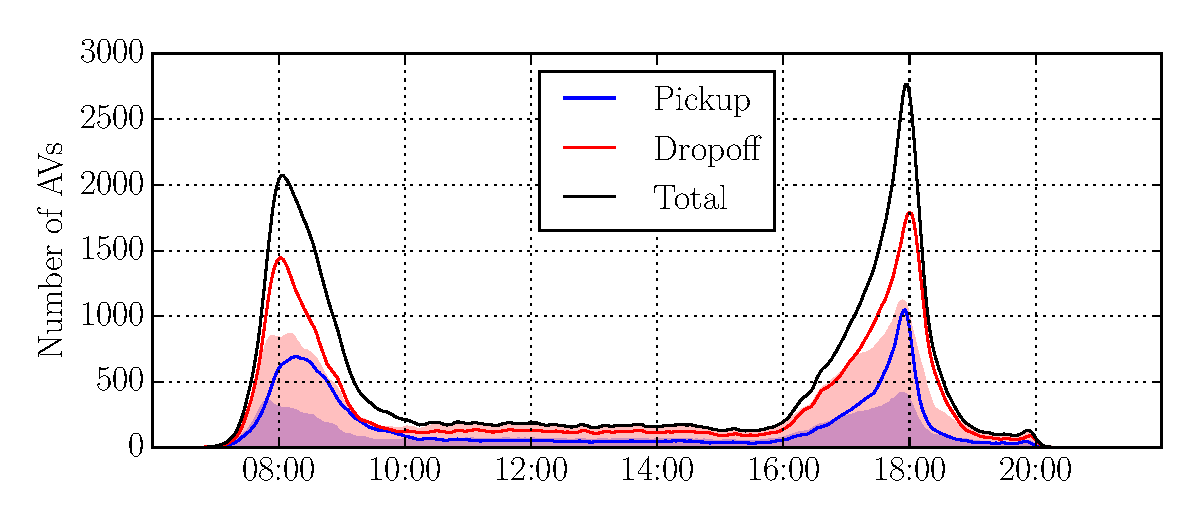
\includegraphics[width=1.0\textwidth]{figures/avwork.pdf}
    \caption{\todo{todo}}
    \label{fig:avwork}
\end{figure}

\subsection{Sensitivity Analysis}

Intuitively, the behaviour of the utility parameters should be quite clear: If
the utility is increased, the AV mode gets more favorable, if it is decreased, less
people will use it. However, in such a complex traffic system there are secondary
effects, which influence the adaptation of AVs. In the following first the general
influence of the single parameters will be discussed and limiting cases will examined.
